

\documentclass{beamer}

\usepackage[utf8]{inputenc}
\usepackage[normalem]{ulem}
\usepackage[T1]{fontenc}
\usepackage{lmodern}
\usepackage{hyperref}
%\usepackage[latin1]{inputenc}
%\usepackage[cyr]{aeguill}
%\usepackage[english]{babel}
\setbeamertemplate{caption}{\raggedright\insertcaption\par} 
\addtobeamertemplate{navigation symbols}{}{%
\usebeamerfont{footline}%
\usebeamercolor[fg]{footline}%
\hspace{1em}%
\insertframenumber
}
%\addtobeamertemplate{footline}{\vspace{30pt}}{\vspace{-30pt}}

%\expandafter\def\expandafter\insertshorttitle\expandafter{%
 % \insertshorttitle\hfill%
  %\insertframenumber\,/\,\inserttotalframenumber}

\begin{document}
\title{O2 DQ framework tutorial introduction: idea, structure and running
%  \\[3\baselineskip]
}  
\setbeamercolor{item projected}{bg=red}
\setbeamertemplate{enumerate items}[default] 
\setbeamercolor{frametitle}{fg=red}
\setbeamercolor{title}{fg=red}
\setbeamercolor{structure}{fg=red}
\setbeamercolor{section in sidebar}{fg=red}
\setbeamercolor{frametitle}{fg=red}
\setbeamercolor{block title}{fg=red}
\setbeamercolor{local structure}{fg=red}
\setbeamercolor{section}{fg=red}
\setbeamercolor{enumerate}{fg=red}
\setbeamertemplate{footline}[frame number]{}
\setbeamertemplate{navigation symbols}{}
\definecolor{forestgreen}{rgb}{0.13, 0.55, 0.13}
\definecolor{darkblue}{rgb}{0.0, 0.0, 0.55}

\addtobeamertemplate{footline}{ \vspace{-1.2cm} \hspace{2cm} Michael Winn (Irfu/CEA), Quarkonia as Tools, 28.04.2023 %\vspace{-3.0cm}
}
 
%\beamertemplatenavigationsymbolsempty
%\setbeamertemplate{footline}[frame number]{}
%\vspace{-5cm}

\author{
  Michael Winn %\\  on behalf of the LHCb Collaboration
} 
\institute{\small Department of Nuclear Physics IRFU/CEA, university Paris-Saclay \\ %\\[\medskipamount]
  nearly exclusively based on material by Ionut Arsene (University of Oslo)
}
\titlegraphic{%\vspace{-6cm}
%  \includegraphics[width=100px]{logomedium}
  
\vspace{8px}

\includegraphics[width=0.3\textwidth,height=.15\textheight]{logosCEAetIrfu_144.png}
%\includegraphics[width=0.6\textwidth]{logo.jpg}
}
\date{
  O2 Tutorial DQ session, 28.04.2023
}


{
  \setbeamertemplate{navigation symbols}{}
  \setbeamertemplate{footline}[frame number]{}
  \setbeamertemplate{footline}{}
   
  \frame{

    \titlepage} 
}

%\addtocounter{framenumber}{-1}

%\frame{\frametitle{Table of contents}\tableofcontents} 
\frame{
  \frametitle{Further detailed material and support}
  \begin{itemize}
    \setlength\itemsep{1em}
  \item Today only a short presentation to allow you to work with the framework
  \item detailed presentation by Ionut and others in DQ meeting in 05/2022~\textcolor{blue}{\href{https://indico.cern.ch/event/1158954/}{link}}
  \item materialin last DQO2 tutorial~\textcolor{blue}{\href{https://indico.cern.ch/event/1220887/}{link}}  
  \item please subscribe to \textcolor{blue}{\href{alice-pwg-DQ-O2@cern.ch}{alice-pwg-DQ-O2@cern.ch}}
  \item in case of further questions beyond the tutorial, use mattermost channel: ´O2-DQ Analysis Framework Alpha´ 
  \end{itemize}
}

\frame{
  \frametitle{Idea and scope of framework}
  \footnotesize
  \begin{itemize}
  \item Idea: all analyses with single or dileptons (electrons \& muons) as part of the analyses
  \item dilepton $+$ 1/2 track(s) (correlations and b-decays), flow measurements, multiplicity dependence measurements,..\\
  \item hence: scope DQ, EM dileptons, single-lepton based HF analyses, could be extended to UD
  \item realised via modularized derived data
  \item embedded in a hierarchical running strategy
  \end{itemize}
}

\frame{
  \frametitle{The O2 DQ Data model}
  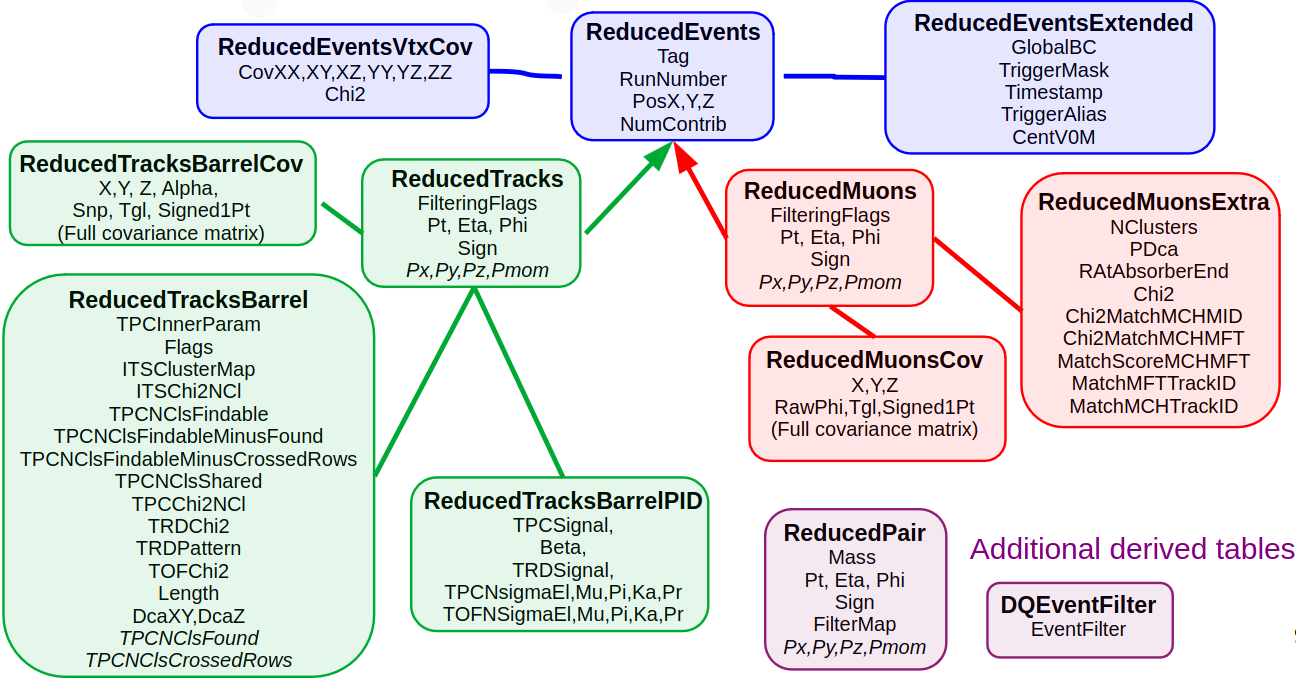
\includegraphics[width=1.05\textwidth]{DataModel.png}
  }

\frame{
  \frametitle{The O2 DQ Data model: MC labelling}
  \begin{figure}
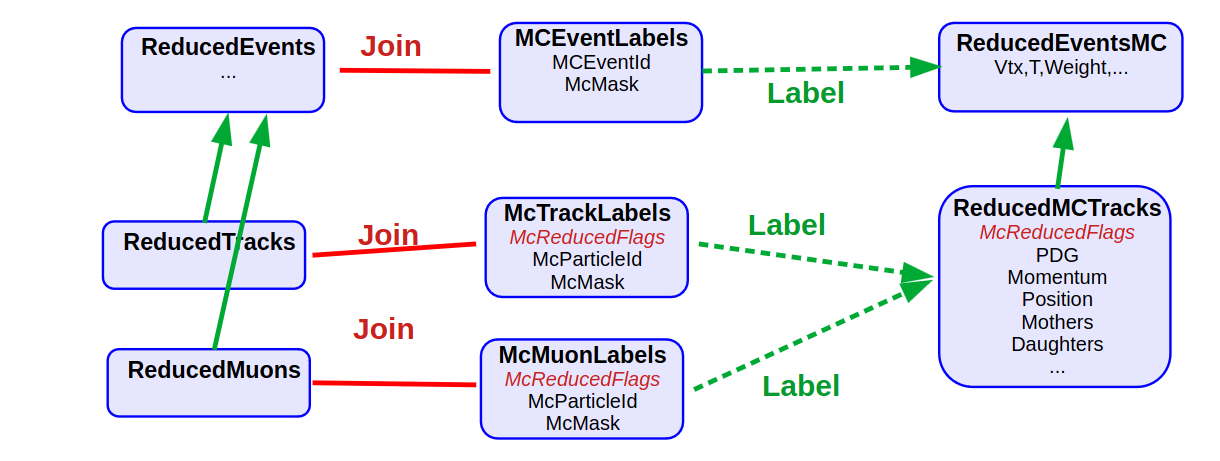
\includegraphics[width=1.05\textwidth]{DataModel_MC.png}
  \end{figure}
  \footnotesize
  \begin{itemize}
  \item MC generator level information can be retrieved via MC "labels", joinable to the event, track and muon tables
  \item Using a skimmed MC model allows for large data size reduction (work with just particles of interest)
    \end{itemize}
  
  }

\frame{
\frametitle{Running philosphy}
\footnotesize
\begin{itemize}
\item Run 3: large data volumes implied by increase of luminosity and ALICE high-granularity detectors
\item 2-3 levels of data reduction within framework to provide relatively small size output including all information needed for analysis with full luminosity
\item trigger layer processing using \textbf{filter-pp}: filter-pp-task (software trigger), based on simple, inclusive single and dilepton signatures
\item centralised hyperloop for derived data with \textbf{table-maker}:  reading AO2D, writing reducedAod.root
\item user-based running on derived data \textbf{table reader}: reading reducedAod.root, writing trees/histograms to analyse
\item final output contains candidates and auxiliary sets of tracks (V0 tracks, dalitz leptons)
\end{itemize}
}

\frame{
\frametitle{Skimming Workflow}
\begin{figure}
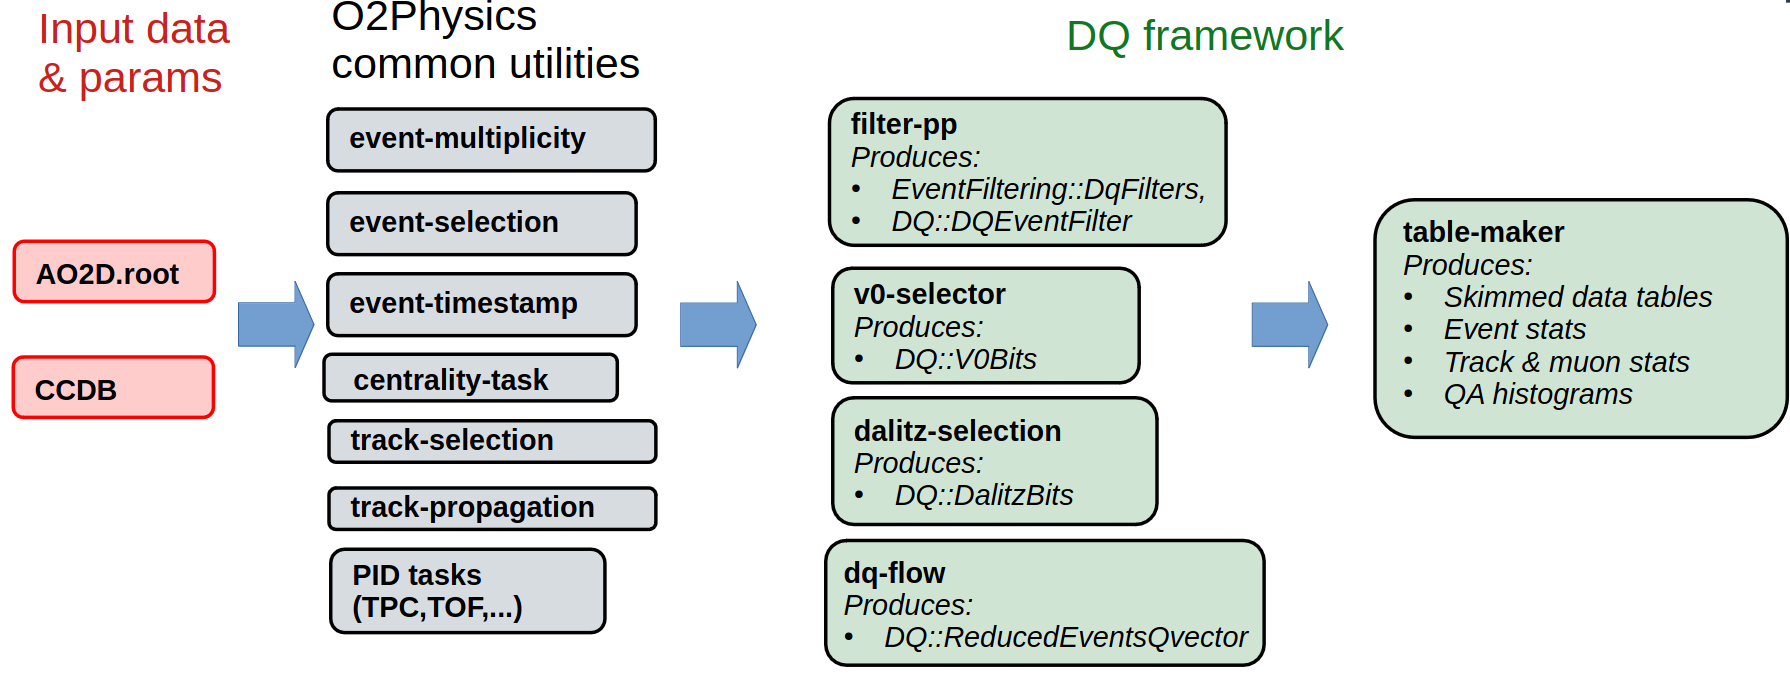
\includegraphics[width=1.05\textwidth]{skimming_workflow.png}
\end{figure}
\footnotesize
\begin{itemize}
\item Produces a "skimmed and slimmed" data model
\item Configurability for\\
  - selecting events, tracks and muons with multiple parallel selections\\
  - Amount of event/track/muon information
\end{itemize}

}

\frame{
  \frametitle{Analysis workflow}
  \begin{figure}
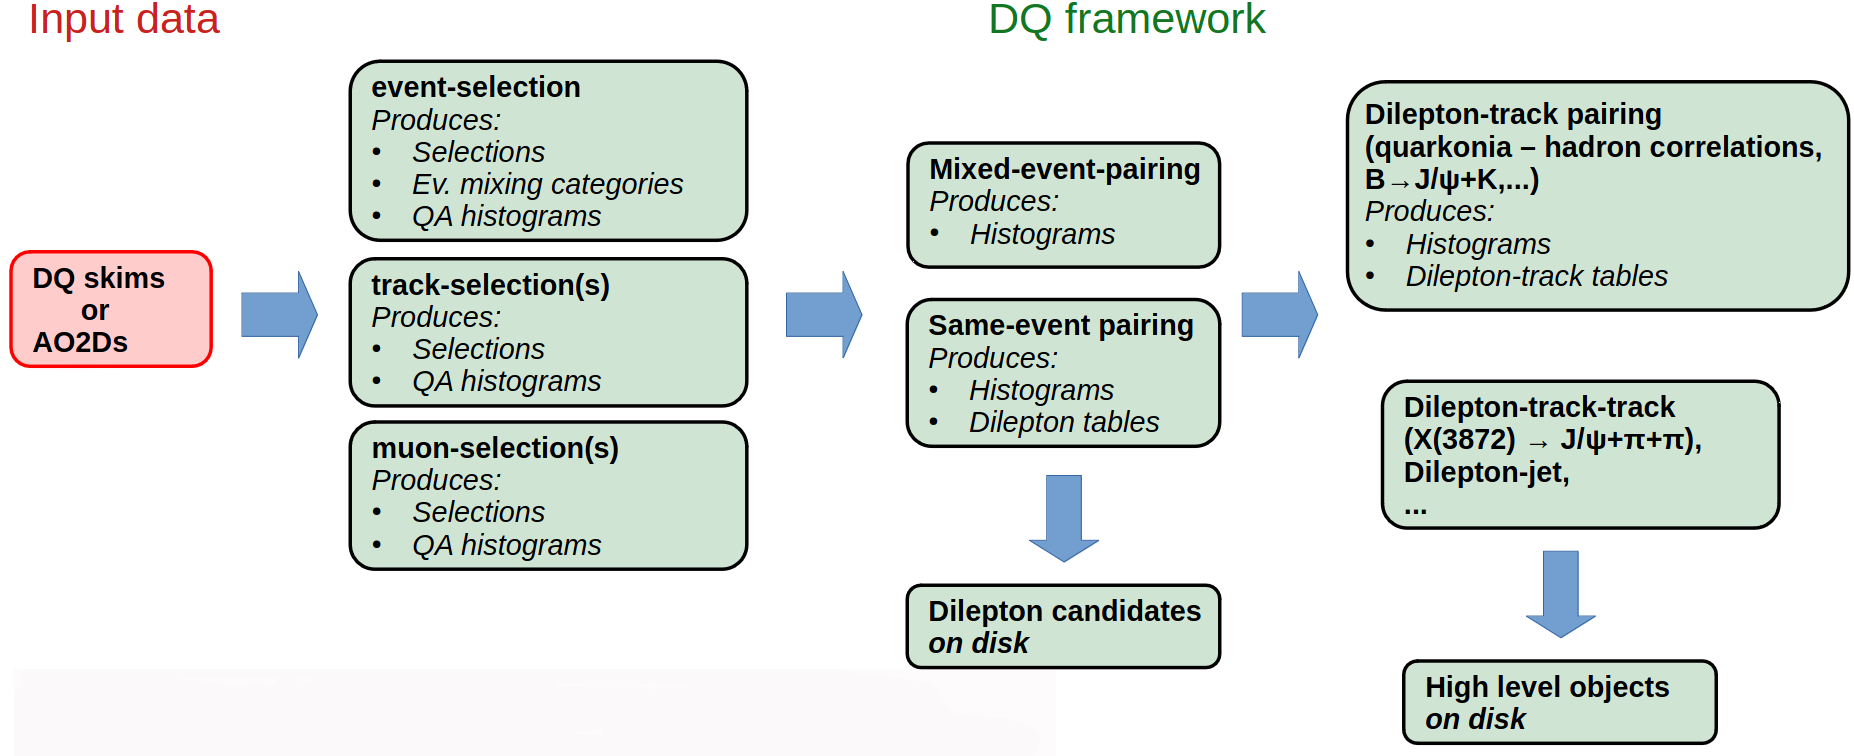
\includegraphics[width=1.05\textwidth]{Analysis_workflow.png}
  \end{figure}
  \footnotesize
  \begin{itemize}
  \item Runs analysis over DQ skims or Framework/AO2D
  \item Can replay event/track selections but also use bits based on decisions computed at skimming time
  \item Produces high level skims for "offline" applications, e.g. machine learning
  \end{itemize}
}

\frame{
  \frametitle{Structure of an analysis task in code}
  \begin{figure}
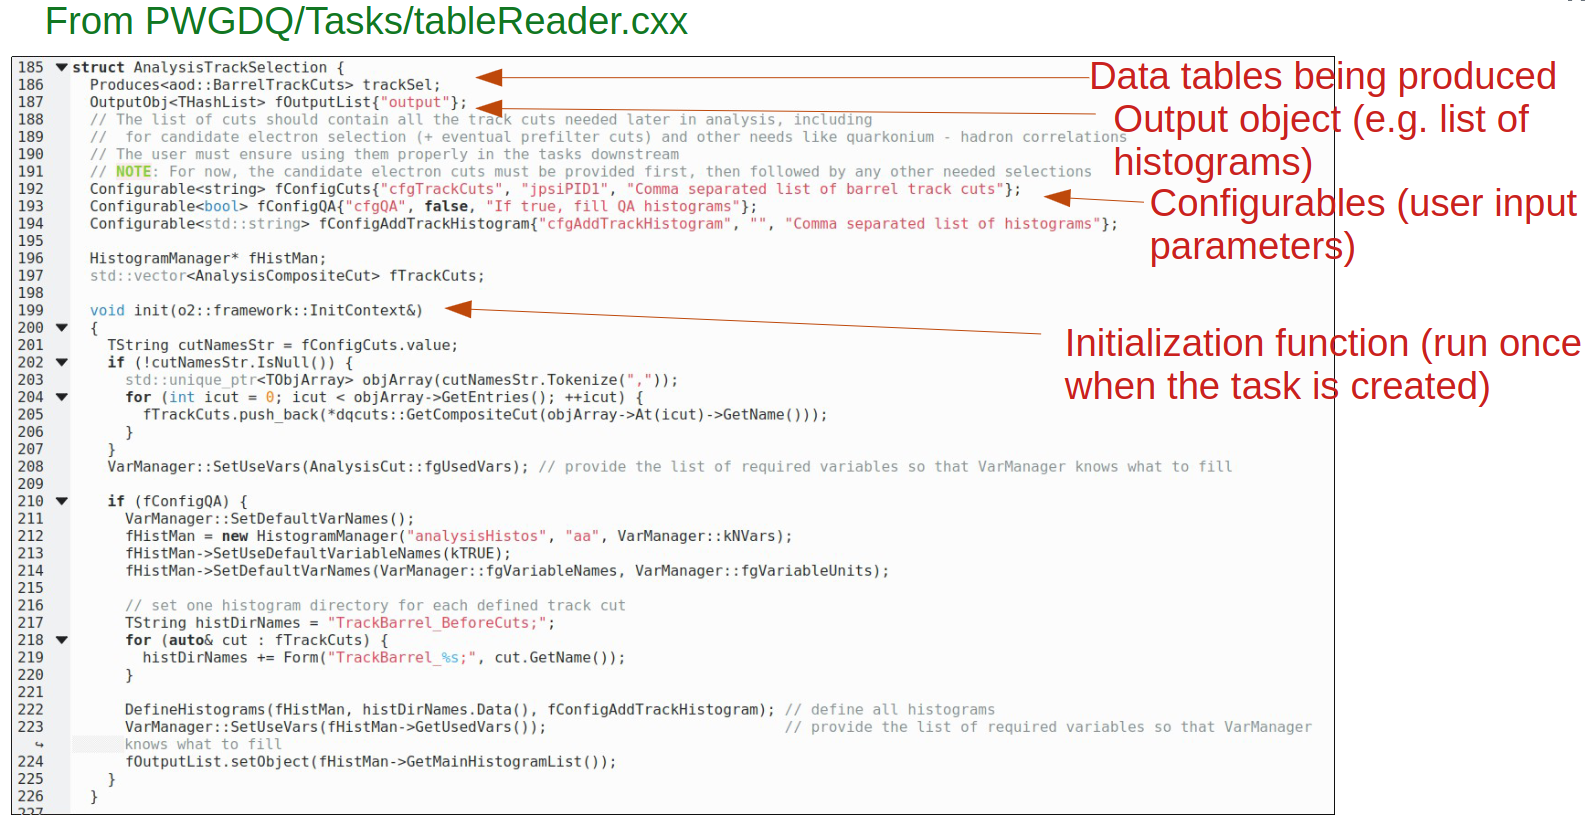
\includegraphics[width=1.05\textwidth]{structure_of_an_analysis_task_in_code.png}
  \end{figure}
}

\frame{
  \frametitle{Structure of an analysis task in code}
  \begin{figure}
    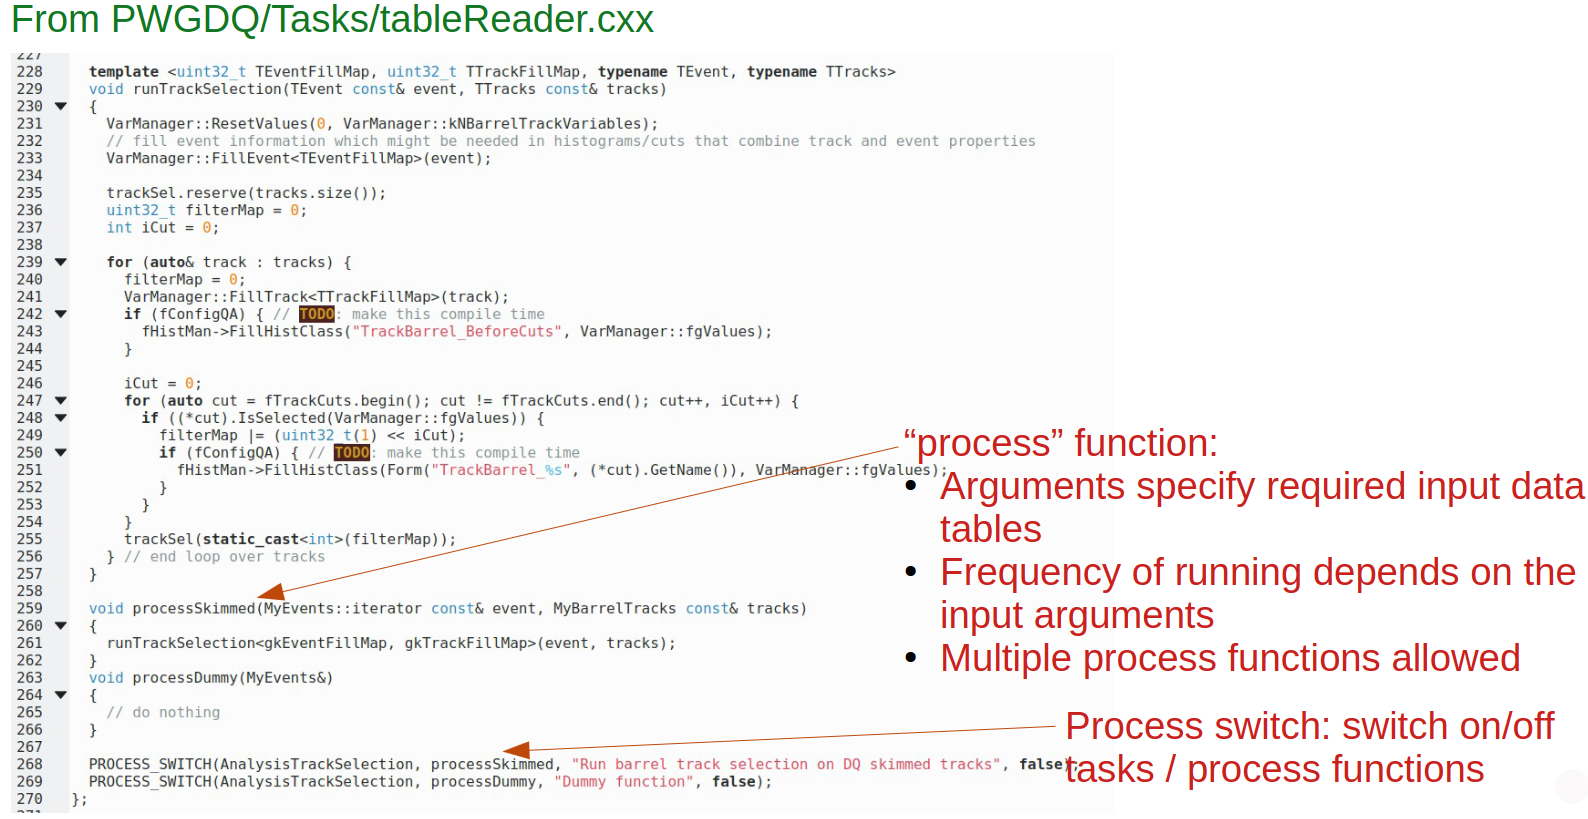
\includegraphics[width=1.05\textwidth]{structure_analysis_task.png}
    \end{figure}
}

\frame{
  \frametitle{Generic structure of workflows in O2}
\footnotesize
  \begin{itemize}
  \item A workflow is a collection of tasks (or DPL devices) running simultaneously in a shared memory environment
  \item  Each task / device must specify:\\
    – Inputs (data tables, other resources)\\
    – Outputs (data tables, histograms, etc)
  \item Can have: \\
    – Specific initialization function: init() \\
    – Configurable input parameters: Configurable \\
    – Other data or function members
  \item  DPL framework organizes/optimizes the chain of running the different tasks based on the specified inputs and outputs
  \end{itemize}
}

\frame{
  \frametitle{Running a workflow in O2}
  \footnotesize
  \begin{itemize}
  \item Main requirements for the user: \\
    – Select the needed tasks to be run in the workflow \\
    – Specify the configuration of each single task / device in the workflow in order to achieve the analysis goals
  \item  Required tasks can be found in the same O2 executable or in different ones \\
    – Multiple O2 executables can be combined in a pipe:\\
    \textcolor{green}{o2-analysis1 | o2-analysis2 | ...}
  \item The user must ensure that the workflow can run, i.e. all needed inputs can be read from input files or can be produced by the specified workflow devices
    \end{itemize}
  }

\frame{
  \frametitle{Running a workflow in O2}
  \footnotesize
  \begin{itemize}
  \item Configuring and running a workflow can be a very laborious and error prone process due to many tasks that usually need to be run, so: \\
    – Task configuration is done using (predefined) \textcolor{red}{.json} files, and \\
    – Workflows are typically run using python scripts
  \item Example of a command line run without the help of scripts:
    - \textcolor{red}{\tiny  o2-analysis-dq-table-maker-mc --configuration json://tempConfig.json --severity error --shm-segment-size 12000000000 --aod-writer-
json aodWriterTempConfig.json -b | o2-analysis-timestamp --configuration json://tempConfig.json -b | o2-analysis-event-selection --
configuration json://tempConfig.json -b | o2-analysis-multiplicity-table --configuration json://tempConfig.json -b | o2-analysis-
trackselection --configuration json://tempConfig.json -b | o2-analysis-pid-tof-base --configuration json://tempConfig.json -b | o2-
analysis-pid-tof --configuration json://tempConfig.json -b | o2-analysis-pid-tof-full --configuration json://tempConfig.json -b | o2-
analysis-pid-tof-beta --configuration json://tempConfig.json -b | o2-analysis-pid-tpc-full --configuration json://tempConfig.json -b | o2-
analysis-track-propagation --configuration json://tempConfig.json -b }
  \item Example of command line using a python script:\\
    - \textcolor{green}{./runTableMaker.py -runMC --arg internal-dpl-aod-reader:aod-file:AO2D.root configTableMakerMCRun3.json --add\_track\_prop}
    \end{itemize}
}

\frame{
  \frametitle{A .json configuration file}
  \begin{columns}                                                                                                                                                                                         
    \begin{column}{0.5\textwidth}    
      \begin{figure}
        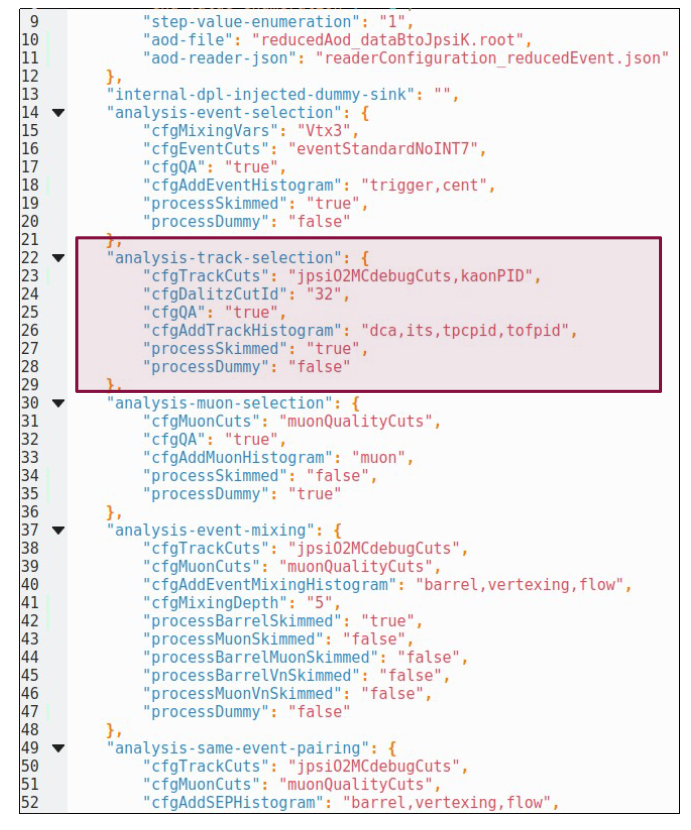
\includegraphics[width=1.\textwidth]{json_configuration.png}
      \end{figure}
    \end{column}
    \begin{column}{0.5\textwidth}                                                                                                                                                                          \footnotesize
      \begin{itemize}                                                                                                                                                                                           \item All tasks in the workflow need to have a specified configuration in .json file
        - Specify the configurables and process functions
      \item See e.g. for the track selection task shown in slides 5-6
      \item  N.B. When a task is included in the workflow, at least one process function must be active
        - Sometime if we want to switch off a task from an executable that is being run, we enable a process function named “processDummy” which does nothing 
      \end{itemize}                                                                                                                                                                                      
\end{column}                                                                                                                                                                                              
\end{columns} 
}



\frame{
\frametitle{A .json reader/writer configuration}
\footnotesize
\begin{columns}
  \begin{column}{0.3\textwidth}
\begin{figure}
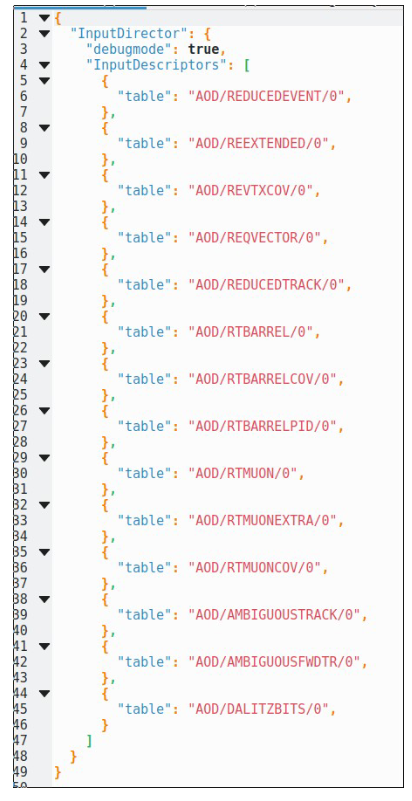
\includegraphics[width=1.0\textwidth]{json_writer_configuration.png}
\end{figure}
  \end{column}
  \begin{column}{0.7\textwidth}
    \footnotesize
    \begin{itemize}
    \item A reader/writer configuration file specifies the data tables to be read from or written to disk \\
      - Needed when one works with data models other than the central O2/Framework model
    \item The file can specify just the table identifier or it can specify detailed information, e.g. customized names for each data member in a table
    \item  These files are typically needed when:\\
      - Analyzing skimmed data
      - Writing skimmed data to disk
    \end{itemize}
    \end{column}
\end{columns}
}

\frame{
  \frametitle{The goals of this tutorial}
  \footnotesize
  \begin{itemize}
  \item Understand the way workflows are configured
  \item  Run data and MC skimming, tailored to your analysis\\
    – Merge the skims into larger data frames (to avoid empty or nearly empty data frames)
  \item Analyze the skims\\
    – Dilepton analysis\\
    – Dilepton $+$ hadron analysis \\
    – Run over MC and match reconstructed and generator level objects
  \end{itemize}
 
}

\end{document}
